\vspace{-0.2cm}
\subsection{Federated Fine-Tuning LMs with LoRA}
\vspace{-0.1cm}
\textbf{Language Models.}
From design to deployment, training transformer-based LMs typically involves two main stages: pre-training and fine-tuning \cite{vaswani2017attention, lin2021fednlp, cai2022fedadapter}.
In the first stage, the LMs are pre-trained on the large-scale corpus, \eg, Wikipedia \cite{wikidump}, C4 \cite{2019t5}, to learn the ubiquitous linguistic structure, which is independent of downstream tasks \cite{cai2022fedadapter}.
The pre-training stage demands massive computing resources, typically undertaken by large tech companies \cite{devlin2018bert, brown2020language}, such as Google and Microsoft.
Fine-tuning adapts the pre-trained LMs to various downstream tasks, such as text classification and text generation, which require substantial data to update the entire LM for a giving task.
% for the given task.
However, fine-tuning the entire LM usually demands excessive resources, \eg, computing and communication resources, leading to slow fine-tuning speeds on resource-constraint devices \cite{cai2022fedadapter, xu2023federated}.

\textbf{LoRA for LMs.}
Herein, low-rank adaptation (LoRA) adds trainable rank decomposition matrices to each transformer layer of the LM while freezing the pre-trained weights of the LM to improve fine-tuning efficiency \cite{hu2021lora}. 
For a pre-trained weight matrix $\mathcal{M} \in \mathbb{R}^{m \times q}$ ($m$ and $q$ are the dimension sizes of $\mathcal{M}$), LoRA injects low-rank decomposition $\Delta \mathcal{M} = \mathcal{B}\mathcal{A}$ as the trainable parameters. 
Note that, $\mathcal{B} \in \mathbb{R}^{m \times r}$ and $\mathcal{A} \in \mathbb{R}^{r \times q}$ are the project-down matrix and the project-up matrix respectively, where $r$ denotes the rank of LoRA and is much smaller than both $m$ and $q$.
Formally, for a simple linear layer $y = \mathcal{M}x$ in the transformer layer, LoRA modifies the forward propagation as: 
% \vspace{-0.1cm}
\begin{equation}
    y = \mathcal{M}x + \mathcal{B}\mathcal{A}x
    \vspace{-0.1cm}
\end{equation}
where $x \in \mathbb{R}^{q \times s}$ and $y \in \mathbb{R}^{m \times s}$ are the input tensors and the output tensors, respectively, and $s$ is the sequence length (\ie, the number of tokens in a given sequence). 
As a generation of full fine-tuning \cite{hu2021lora}, LoRA utilizes two bypass matrices (\ie, $\mathcal{B}$ and $\mathcal{A}$) with the low rank to perform fine-tuning without modifying the pre-trained weight matrix, thus LoRA can be applied to any transformer layers of the LMs.
Fine-tuning LMs with LoRA can greatly reduce the number of trainable parameters (typically less than 1\% \cite{hu2021lora, zhang2023fedpetuning}) while maintaining satisfactory fine-tuning performance.


\textbf{FedFT with LoRA.}
Considering a distributed system with one PS and $n$ devices, FedFT is proposed to fine-tune the LMs through a loose federation of devices. %coordinated by the PS.
Naturally, LoRA is introduced into FedFT (\eg, FedLoRA) to reduce computing and communication overhead \cite{zhang2023fedpetuning, cho2023heterogeneous}.
The difference between FedFT (\eg, FedNLP) and FedLoRA is illustrated in Figure \ref{fig:illustration}.
FedLoRA only exchanges lightweight LoRA layers $\widetilde{\theta}$ instead of all cumbersome LMs $\overline{\theta}$ in FedFT.
The goal of FedLoRA is to find the optimal model $\theta^* = \{ \widetilde{\theta}^*, \overline{\theta} \}$ minimizing the loss function $f(\theta)$ as follows:
\vspace{-0.2cm}
\begin{equation}
    \min_{\theta = \{ \widetilde{\theta}, \overline{\theta} \}} f(\theta) \triangleq \frac{1}{n} \sum_{i = 1}^{n} f_i(\theta_i)
    \vspace{-0.2cm}
\end{equation}
where $f_i(\theta_i) = \frac{1}{|\mathbb{D}_i|} \sum_{\xi_i \in \mathbb{D}_i} F_i(\theta_i; \xi_i)$ denotes the loss function of the local model $\theta_i$ on device $i$ and $F_i(\theta_i; \xi_i)$ is the loss over data samples $\xi_i$ on local dataset $\mathbb{D}_i$. 
To minimize the local objective function, device $i$ only updates the LoRA layers through the gradient descent algorithm (\eg, AdamW \cite{loshchilov2017decoupled}).
The optimization procedure for updating the LoRA layers $\widetilde{\theta}_i^{h}$ on device $i$ at local step $t$ in round $h$ can be expressed as: 
% \vspace{-0.1cm}
\begin{equation}
    \widetilde{\theta}_i^{h,t} = \widetilde{\theta}_i^{h,t - 1} - \eta \cdot \nabla f_i(\widetilde{\theta}_i^{h, t - 1})
    % \vspace{-0.1cm}
\end{equation}
where $\eta$ is the learning rate and $\nabla f_i(\widetilde{\theta}_i^{h, t - 1})$ is the gradient of the loss for LoRA layers $\widetilde{\theta}_i^{h, t - 1}$.

After local fine-tuning, all devices send the updated LoRA layers to the PS for global aggregation as follows: 
\vspace{-0.1cm}
\begin{equation}
    \widetilde{\theta}^{h+1} = \frac{1}{n} \sum_{i=1}^{n} \widetilde{\theta}_i^h
    \vspace{-0.1cm}
\end{equation}
After global aggregation, the PS distributes the latest LoRA layers to all devices and moves to the next fine-tuning round.
\vspace{-0.3cm}

% \vspace{-0.5cm}
\subsection{Importance of LoRA Position}
\vspace{-0.1cm}
\label{lora-position}
Existing LoRA-based frameworks (\eg, FedLoRA \cite{zhang2023fedpetuning} and HetLoRA \cite{cho2023heterogeneous}) typically add LoRA layers to all transformer layers, which requires the complete backpropagation process to update all LoRA layers \cite{kaddour2023challenges} and results in a slow convergence rate for fine-tuning pre-trained LMs on resource-constrained devices.
As illustrated in Figure \ref{illu-bert}, we divide an LM (\eg, RoBERTa) into three parts representing different positions, \ie, shallow, medium and deep, respectively.
Based on the backward direction of the backpropagation process, fine-tuning the continuous LoRA layers added to the transformer layers at deep position is computationally efficient while achieving satisfactory fine-tuning performance. 
Wei \etal \cite{wei2024flexora} provide rigorous theoretical insights into the convergence of partial LoRA layer fine-tuning.
Besides, only the LoRA layers at deep position need to perform the backpropagation process and be transmitted to the PS, effectively reducing computing/communication overhead and speeding up the fine-tuning process.
In addition, since pre-trained LMs have acquired powerful language understanding and generation capabilities during the pre-training stage, fine-tuning the added LoRA layers to partial transformer layers at deep position can essentially achieve comparable fine-tuning performance \cite{guo2019spottune, lin2021fednlp, zhang2023adaptive}. 

% \bluenote{
% Besides, fine-tuning the added LoRA layers at deep position effectively leverages the strong language understanding and generation capabilities of the shallow transformer layers in the pre-trained LMs, achieving comparable fine-tuning performance \cite{guo2019spottune, lin2021fednlp, zhang2023adaptive, wei2024flexora}. 
% }
% \rednote{
% This is theoretically supported by Wei \etal \cite{wei2024flexora}, who proved that optimizing a subset of LoRA layers is sufficient to achieve comparable fine-tuning performance. 
% }
% \bluenote{
% Besides, since pre-trained LMs have acquired powerful language understanding and generation capabilities during the pre-training stage \cite{devlin2018bert, liu2019roberta}, fine-tuning the added LoRA layers to partial transformer layers at deep position can essentially achieve comparable performance \cite{wei2024flexora, guo2019spottune, lin2021fednlp, zhang2023adaptive}. 
% This is theoretically supported by the hierarchical learning nature of deep neural networks, where deeper layers are more task-specific and adaptable while preserving the general language understanding capabilities learned in earlier layers \cite{alom2019state}.
% }
% \bluenote{
% Besides, the hierarchical learning nature of deep neural networks: shallow layers extract general token-level features, while deeper layers encode task-specific sentence-level semantics.
% given that pre-trained LMs possess strong language understanding and generation capabilities, fine-tuning only the LoRA layers in deeper transformer blocks can achieve comparable performance \cite{wei2024flexora, guo2019spottune, lin2021fednlp, zhang2023adaptive}. 
% This aligns with the hierarchical nature of deep neural networks, where deeper layers specialize in task-specific features while earlier layers maintain fundamental linguistic knowledge.
% }


To demonstrate the importance of LoRA position, we conduct a set of experiments for federated fine-tuning RoBERTa \cite{liu2019roberta} on SST-2 \cite{wang2018glue} with 10 devices (more experimental setup details in Section \ref{evaluation}).
We train a 12-layer RoBERTa with LoRA layers added to partial transformer layers at different positions (as illustrated in Figure \ref{illu-bert}), including all layers (denoted as \textit{Layers-A}), shallow layers \{\#0, \#1, \#2, \#3\} (denoted as \textit{Layers-S}), medium layers \{\#4, \#5, \#6, \#7\} (denoted as \textit{Layers-M}), and deep layers \{\#8, \#9, \#10, \#11\} (denoted as \textit{Layers-D}).
As shown in Figure \ref{ob-1}, we can derive the following conclusions:

1) Fine-tuning LoRA layers added to only the transformer layers at the deep position achieves comparable performance to vanilla LoRA.
For example, as shown in Figure \ref{1a}, Layers-D achieves comparable final accuracy (\ie, 93.1\%) to Layers-A (94.3\%), with only fine-tuning a third of LoRA layers in Layers-A (\ie, less computing resource). In addition, compared with Layers-S and Layers-M, Layers-D improves the final model accuracy by 6.4\% and 1.3\%, respectively.
% total rank is the same

\begin{figure}[t]
    \centering
    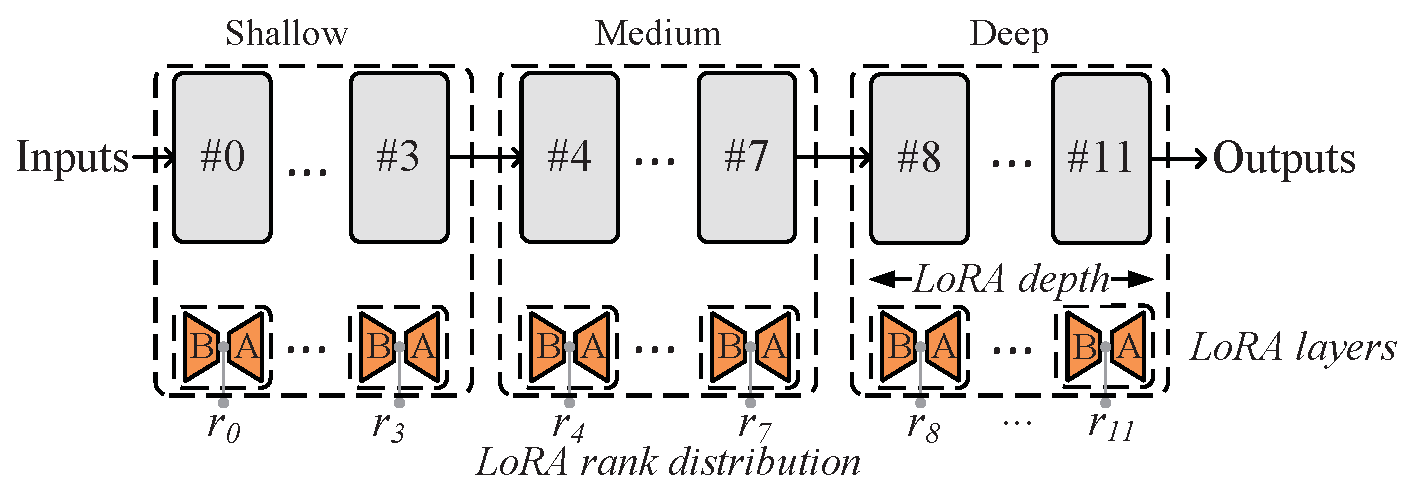
\includegraphics[width=1.0\columnwidth]{figs/position.eps}
    \vspace{-0.7cm}
    \caption{Fine-tuning RoBERTa at different positions.
    }
    \label{illu-bert}
    \vspace{-0.4cm}
\end{figure}

2) Fine-tuning LoRA layers added to only the transformer layers at deep position speeds up the fine-tuning process. 
For instance, by Figure \ref{1b}, Layers-D achieves 2.1$\times$, 1.6$\times$, and 1.2$\times$ speedup compared to Layers-A, Layers-S, and Layers-M, respectively.
This is because Layers-D greatly shortens the backpropagation process from 12 transformer layers to 4 transformer layers, reducing the fine-tuning time.

By the results, the LoRA position will greatly affect fine-tuning performance and resource consumption, while adding LoRA layers to a fixed number of transformer layers at the deep position can save resource cost with satisfactory fine-tuning performance.
Our conclusion is consistent with the relevant conclusions that layers at the deep position are more important than those at the shallow position \cite{zhang2022adaptive, cai2022fedadapter, zhu2023pockengine}.
\vspace{-0.3cm}

% \begin{figure}[t]
%     \centering
%     \subfigure[Test accuracy]{
%         \begin{minipage}[t]{0.5\linewidth}
%         \centering
%         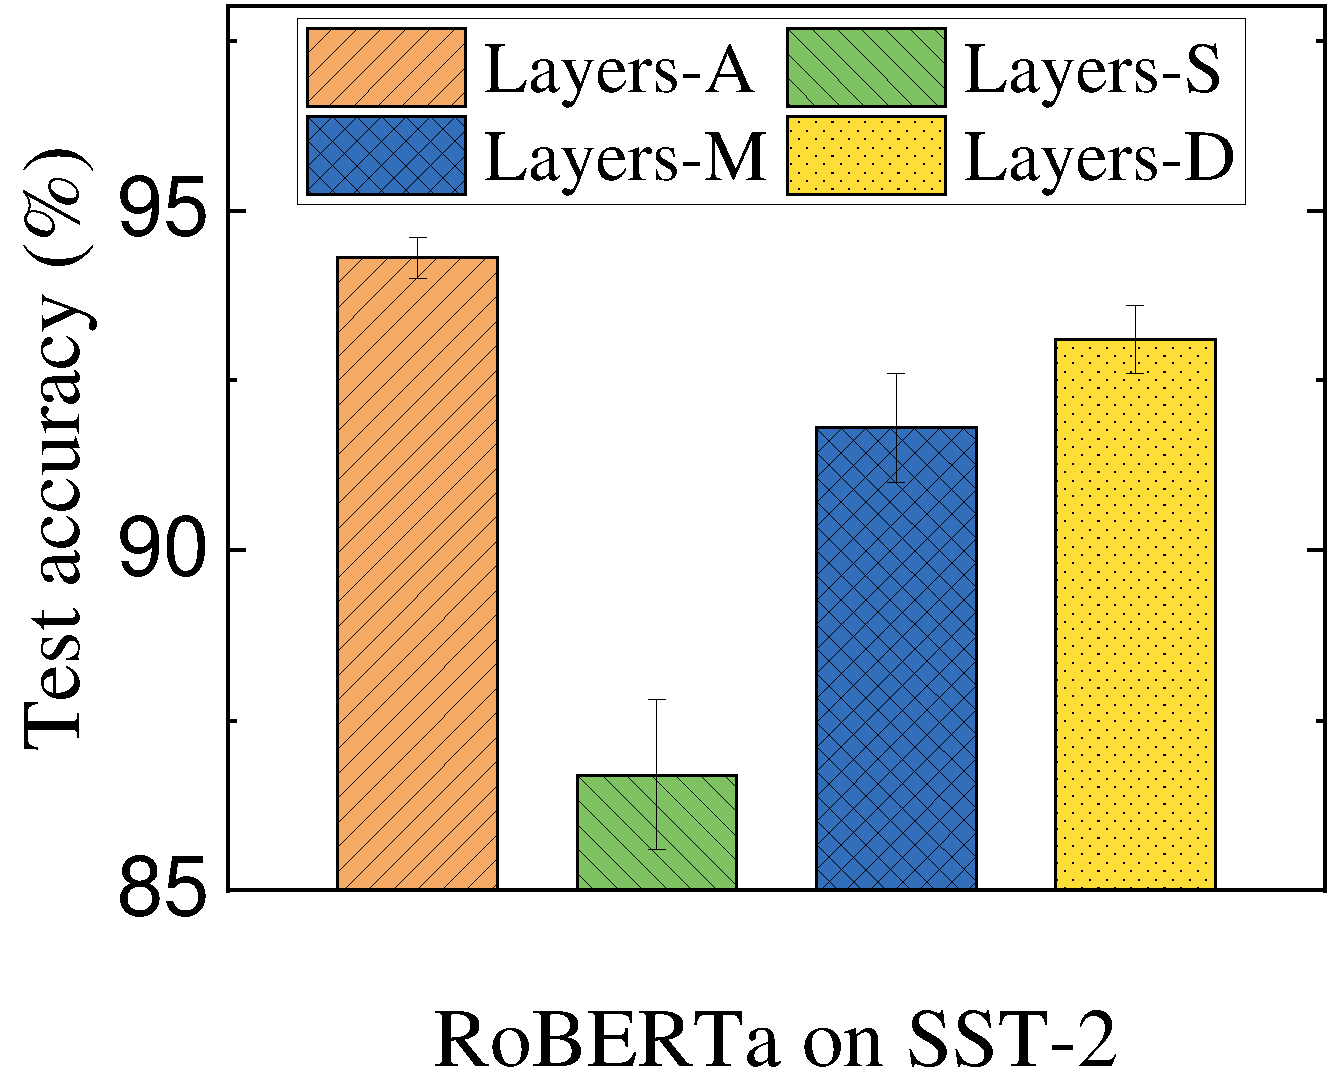
\includegraphics[width=1.7in]{figs/top-layer-rank-more-important-1.pdf}
%         \end{minipage}%
%         \label{1a}
%     }%
%     \subfigure[Per-batch latency]{
%         \begin{minipage}[t]{0.5\linewidth}
%         \centering
%         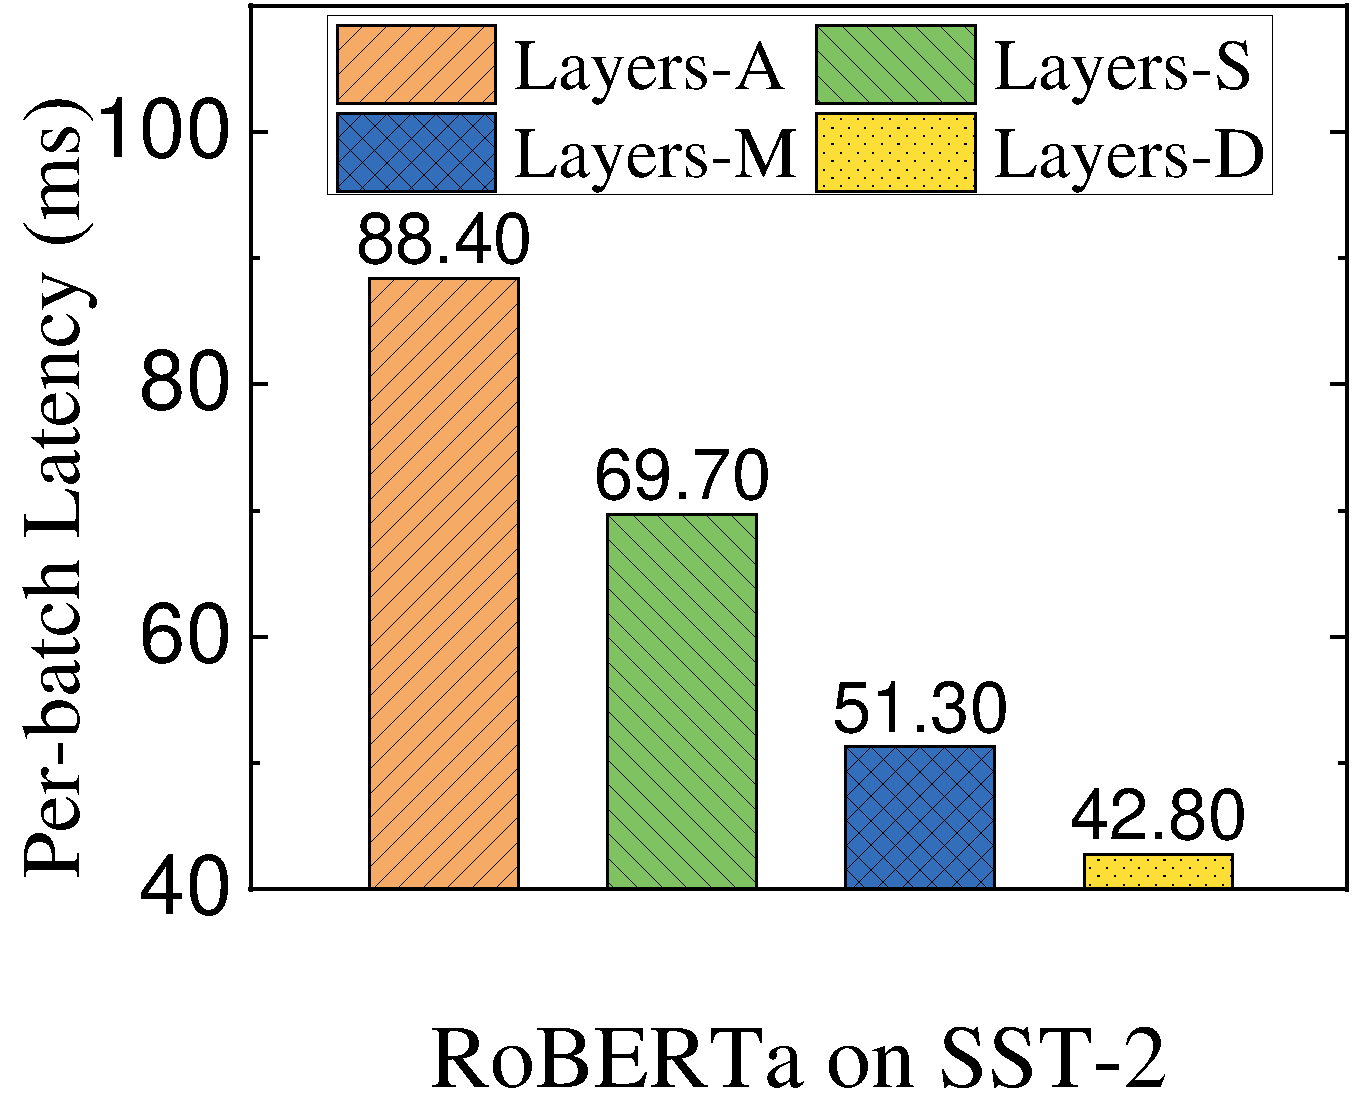
\includegraphics[width=1.7in]{figs/memory-speed-diff-alloc.pdf}
%         \end{minipage}%
%         \label{1b}
%     }%
%     \centering
%     \vspace{-0.5cm}
%     \caption{The impact of position.}
%     \label{ob-1}
%     \vspace{-0.6cm}
% \end{figure}

% \begin{figure}[t]
%     \centering
%     \subfigure[Accuracy loss \& Per-batch latency]{
%         \begin{minipage}[t]{0.5\linewidth}
%         \centering
%         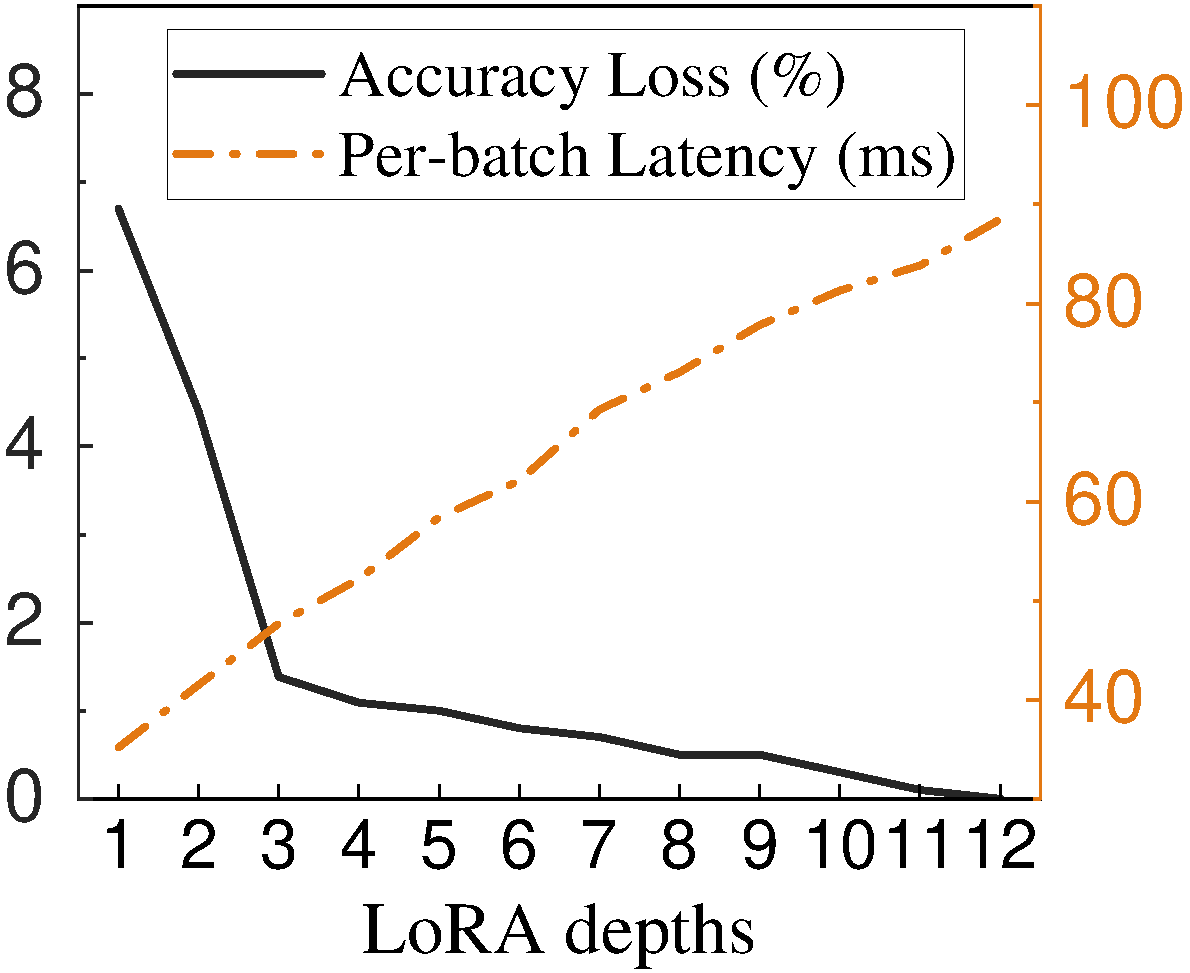
\includegraphics[width=1.7in]{figs/depth-impact-performance-speed.pdf}
%         \end{minipage}%
%         \label{2a}
%     }%
%     \subfigure[Memory usage]{
%         \begin{minipage}[t]{0.5\linewidth}
%         \centering
%         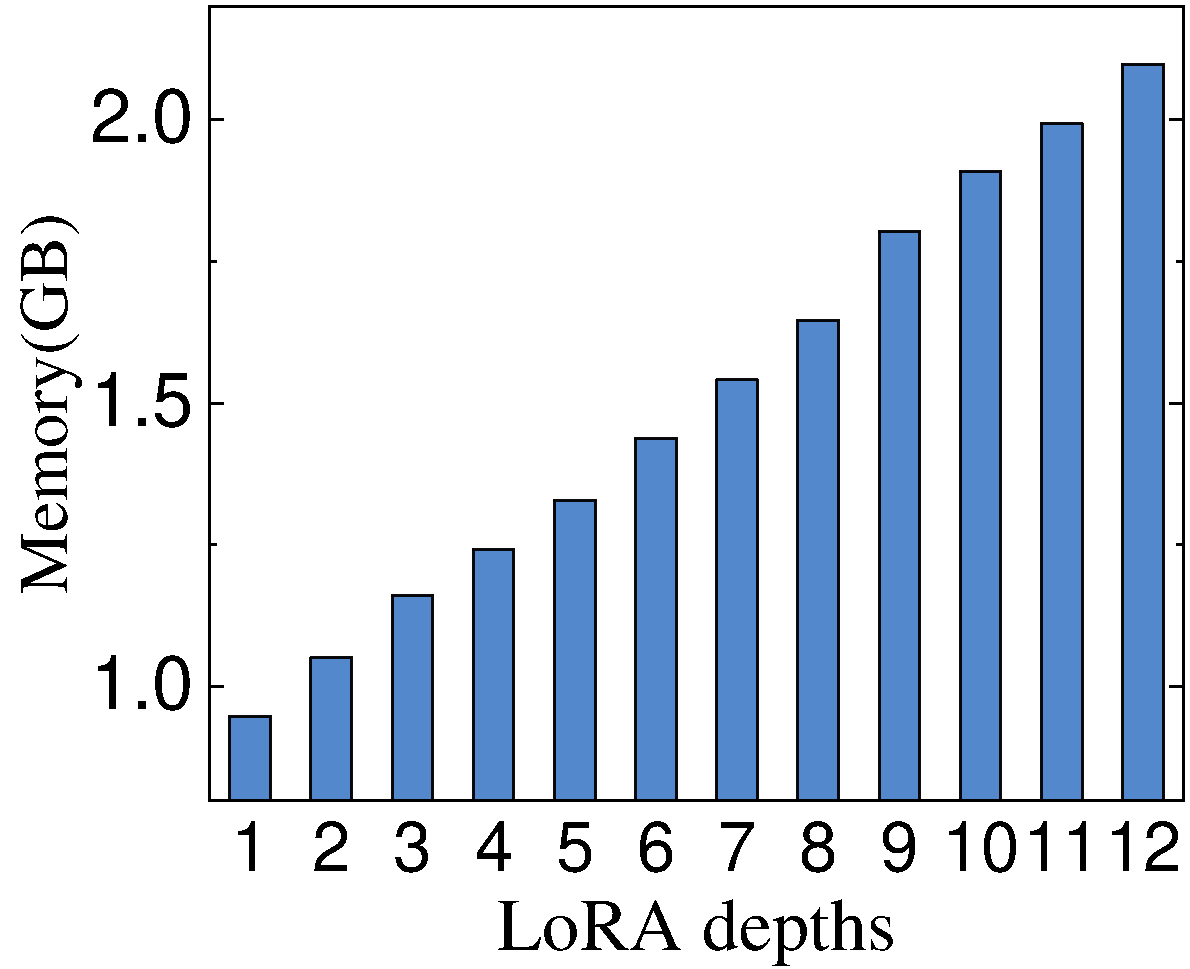
\includegraphics[width=1.7in]{figs/memory-usage.pdf}
%         \end{minipage}%
%         \label{2b}
%     }%
%     \centering
%     \vspace{-0.5cm}
%     \caption{The impact of LoRA depth.}
%     \label{ob-2}
%     \vspace{-0.5cm}
%     % \vspace{-0.3cm}
% \end{figure}

\subsection{Importance of LoRA Depth}
% \vspace{-0.2cm}
\label{lora-depth}
In addition to the results of adding LoRA layers to partial transformer layers at deep position, we further explore the impact of the number of transformer layers at deep position to add extra LoRA layers (called LoRA depth) on fine-tuning performance.
In general, LoRA depth is closely related to fine-tuning performance and resource consumption.
Specifically, the larger LoRA depth means fine-tuning more layers at deep positions to enhance fine-tuning performance but leads to a longer backpropagation process (\ie, slower convergence rate).
Although the smaller LoRA depth can shorten the backpropagation process to speed up the fine-tuning process, it constrains the number of tunable transformer layers and thus restricts the task-fitting capability of the LM.
Therefore, it is critical and non-negligible to determine the appropriate LoRA depth for achieving the trade-off between fine-tuning performance and resource consumption.

\begin{figure}[t]
    % \hspace{-7mm}
    \centering
    \subfigure[Test accuracy]{
        \hspace{-5mm}
        \begin{minipage}[t]{0.5\linewidth}
        \centering
        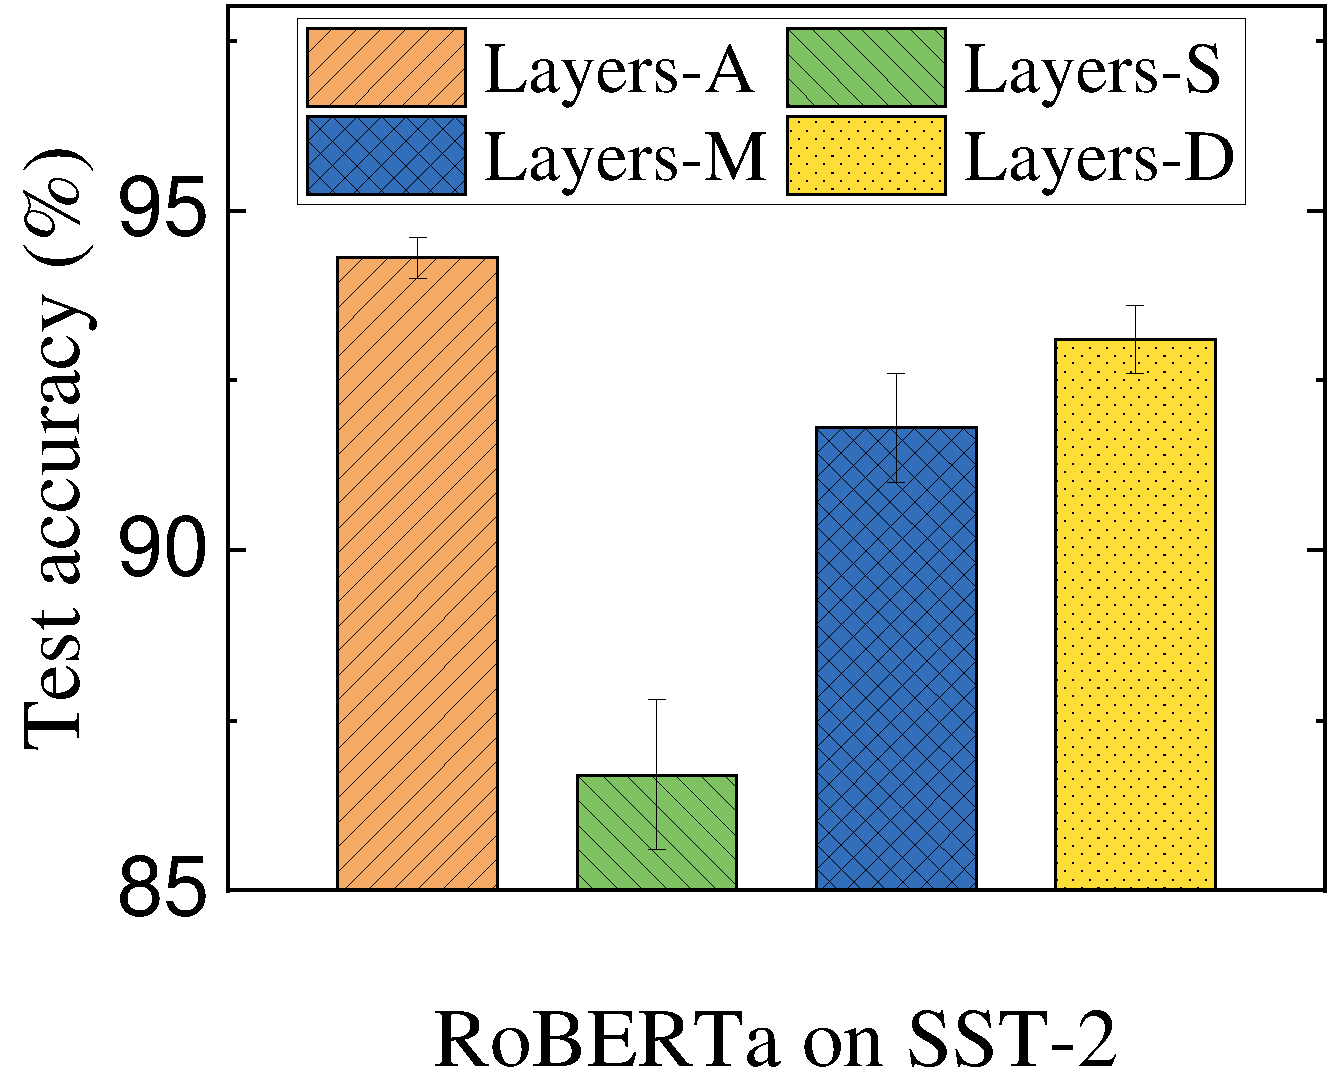
\includegraphics[width=1.6in]{figs/top-layer-rank-more-important-1.pdf}
        \end{minipage}%
        \label{1a}
    }%
    \subfigure[Per-batch latency]{
        \begin{minipage}[t]{0.5\linewidth}
        \centering
        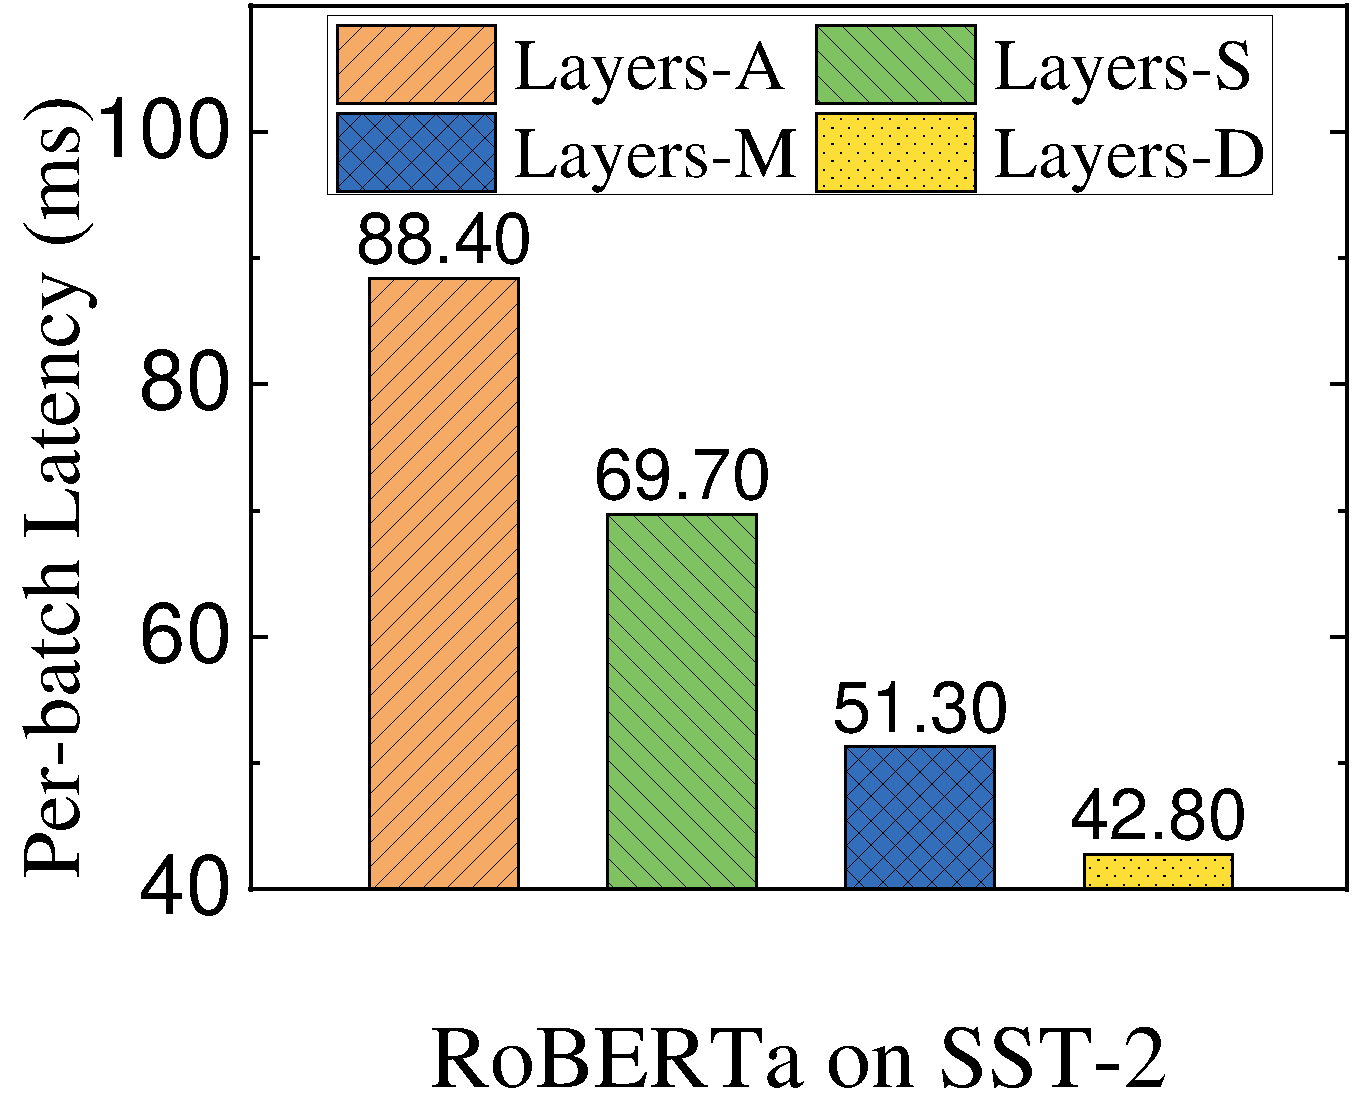
\includegraphics[width=1.6in]{figs/memory-speed-diff-alloc.pdf}
        \end{minipage}%
        \label{1b}
    }%
    \centering
    \vspace{-0.45cm}
    \caption{The impact of LoRA position.}
    \label{ob-1}
    \vspace{-0.2cm}
\end{figure}

\begin{figure}[t]
    \centering
    \subfigure[Accuracy loss \& Per-batch latency]{
        \begin{minipage}[t]{0.5\linewidth}
        \centering
        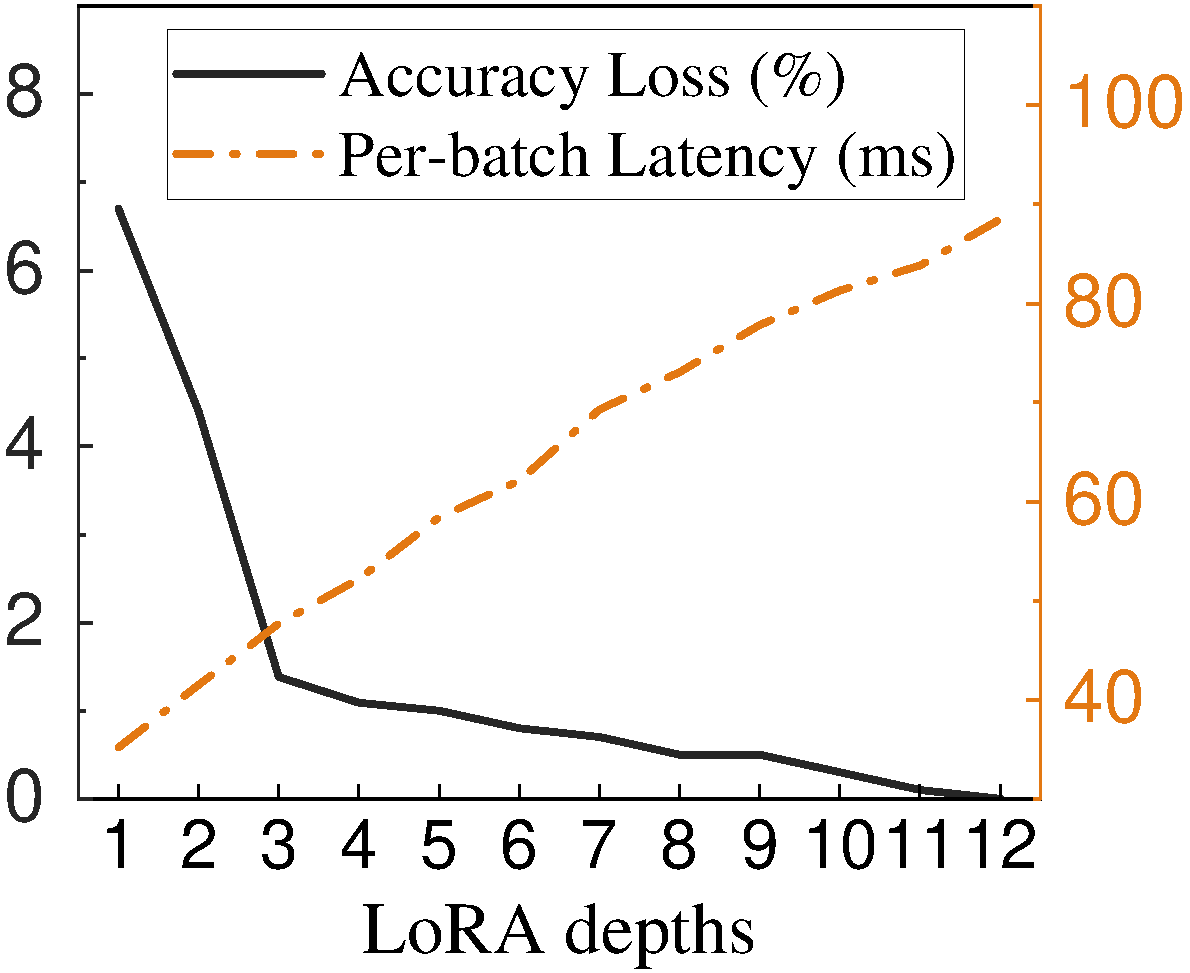
\includegraphics[width=1.6in]{figs/depth-impact-performance-speed.pdf}
        \end{minipage}%
        \label{2a}
    }%
    \subfigure[Memory usage]{
        \hspace{-5mm}
        \begin{minipage}[t]{0.5\linewidth}
        \centering
        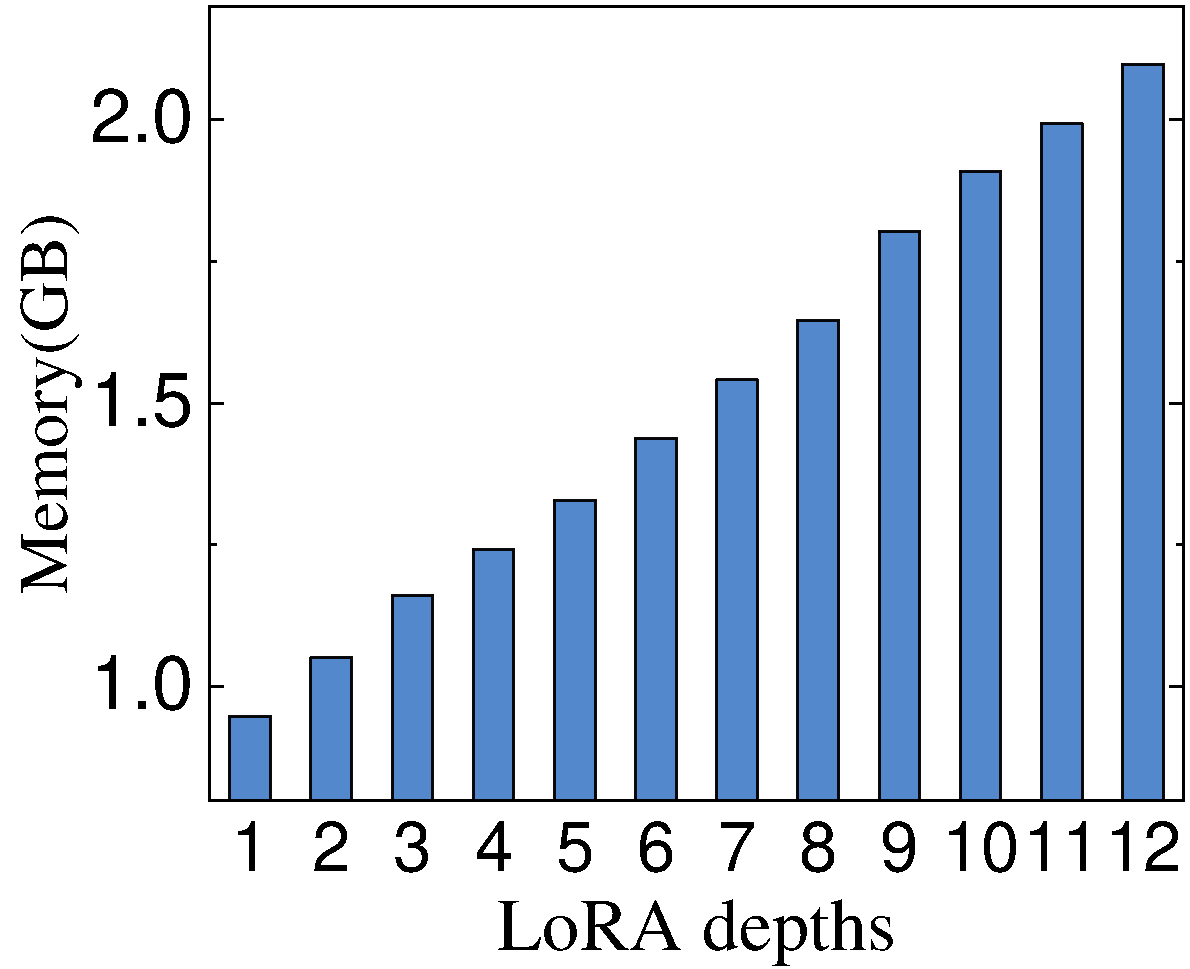
\includegraphics[width=1.6in]{figs/memory-usage.pdf}
        \end{minipage}%
        \label{2b}
    }%
    \centering
    \vspace{-0.5cm}
    \caption{The impact of LoRA depth.}
    \label{ob-2}
    \vspace{-0.4cm}
    % \vspace{-0.3cm}
\end{figure}

To illustrate the impact of the LoRA depth, we conduct a set of experiments for fine-tuning RoBERTa on SST-2 with different LoRA depths (from 1 to 12) and rank of 8. 
We can draw the following conclusions from Figure \ref{ob-2}:

1) As LoRA depth increases, resource consumption (\eg, memory usage) increases almost linearly, resulting in slow convergence rate.
For example, by Figures \ref{2a} and \ref{2b}, with each additional LoRA layer, the per-batch latency increases by approximately 5ms, and the memory usage increases by approximately 107MB. 
Compared with LoRA depth of 1, fine-tuning RoBERTa with depth of 12 results in a 252\% increase in per-batch latency and 221\% growth in memory usage. 

2) The fine-tuning performance improves with the increase of LoRA depth, but the magnitude of the improvement diminishes gradually.
For instance, by Figure \ref{2a}, compared to the LoRA depth of 3, fine-tuning RoBERTa with LoRA depths of 6 and 9 exhibit improvements of 0.6\% and 0.9\% in accuracy, respectively.
As LoRA depth increases from 1 to 3, the final model performance improves by 5.3\%, but only 1.4\% from LoRA depth of 3 to 12.

By the results, carefully determining LoRA depth is critical to improve fine-tuning performance while saving computing and communication resources.
Moreover, to deal with system heterogeneity, LEGEND assigns different LoRA depths for heterogeneous devices to adapt their capabilities.
The devices with strong computing and communication capabilities are assigned with larger LoRA depths, while those with lower computing and communication capabilities are assigned with smaller LoRA depths, so as to reduce waiting time and further improve fine-tuning efficiency.
\vspace{-0.3cm}

\begin{figure}[t]
    \hspace{-3mm}
    \centering
    \subfigure[Performance gain (rank 1 $\rightarrow$ 128)]{
        \begin{minipage}[t]{0.5\linewidth}
        \centering
        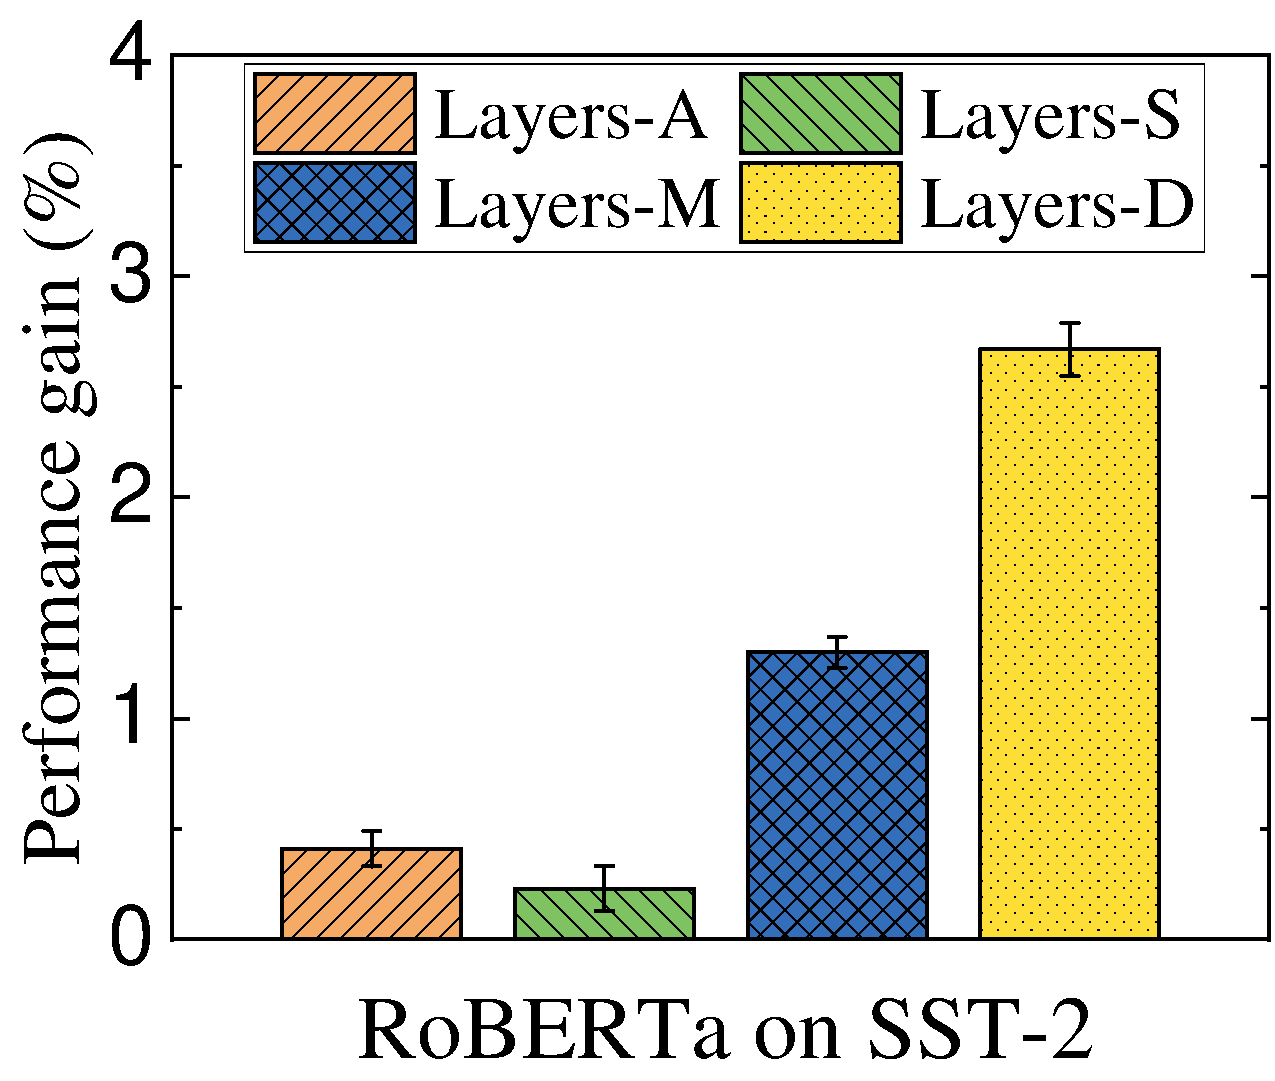
\includegraphics[width=1.62in]{figs/top-layer-rank-more-important.pdf}
        \end{minipage}%
        \label{3a}
    }%
    \subfigure[Final accuracy]{
        \begin{minipage}[t]{0.5\linewidth}
        \centering
        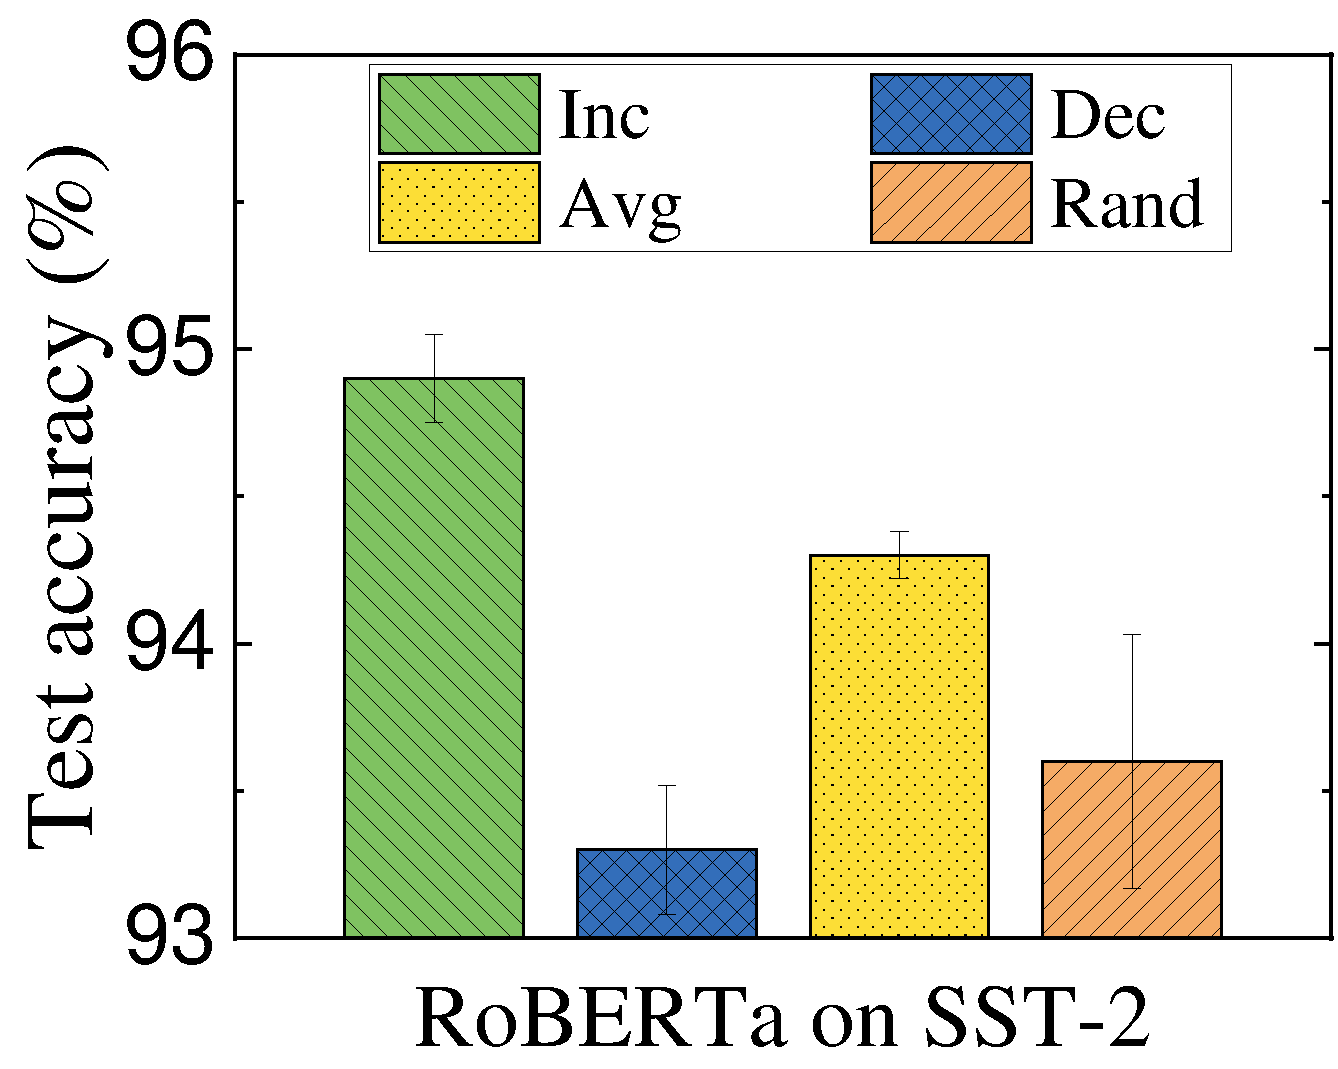
\includegraphics[width=1.7in]{figs/fina_acc_bert_sst2_rank-distribution.pdf}
        \end{minipage}%
        \label{3b}
    }%
    \centering
    \vspace{-0.5cm}
    \caption{The impact of LoRA rank distribution.}
    \label{ob-3}
    \vspace{-0.4cm}
% \vspace{-0.3cm}
\end{figure}

% \vspace{-0.2cm}
\subsection{Importance of LoRA Rank Distribution}
% \vspace{-0.2cm}
\label{lora-distribution}
% We further explore the impact of rank distribution on the fine-tuning performance.
% Specifically, the higher ranks of the deep LoRA layers achieve better fine-tuning performance on a specific task, since the layers at deep position need to focus on higher semantic levels and more contextual information \cite{gao2024higher}.
% Besides, relatively shallow LoRA layers with smaller ranks will leverage the pre-trained LM's inherent capability to extract content information to prevent over-fitting and achieve satisfactory model performance.
We further explore the impact of rank distribution on fine-tuning performance. 
In general, the rank of LoRA layer is closely related to the model capacity, and increasing rank is essential for better performance \cite{song2024increasing, shuttleworth2024lora}. 
Given a fixed total rank budget under resource constraints, strategically allocating higher ranks to task-relevant layers becomes crucial for maximizing model performance \cite{zhang2022adaptive, cho2023heterogeneous}.
Specifically, the higher ranks of the deep LoRA layers achieve better fine-tuning performance on a specific task, since the layers at deep position need to focus on higher semantic levels and more contextual information \cite{lin2021fednlp, ma2022layer, liu2023yoga, gao2024higher}. 
Shallow LoRA layers with smaller ranks leverage the pre-trained model's inherent feature extraction capability, preventing overfitting while maintaining model performance. 
% Besides, due to system heterogeneity, only powerful devices can train shallow layers, while deep layers are trainable across all devices. 
% Allocating higher ranks to deep LoRA layers facilitates better model aggregation through increased parameterization, compared to uniform rank distribution.


% \rednote{
% Given the limited resources, we can only add LoRA layers with a specified total rank budget. 
% The parameter efficiency of LoRA also raises limitations on the model capacity. 
% To unlock superior performance, a crucial imperative emerges: elevating the rank of LoRA layers.
% The importance of weight matrices varies significantly across layers when fine-tuning pre-trained LMs.
% Deeper layers should be allocated higher ranks than the shallower layers. 
% More ranks with fine-grained processing on token-level information may introduce redundancy. 
% On the contrary, deeper layers require high ranks because deeper layers learn more
% abstract and high-level information. 
% More ranks can enhance the LM's capacity to learn fine-grained and task-specific patterns for complicated downstream problems \cite{gao2024higher}.
% Thus, allocating higher ranks to task-critical layers (\eg, deep LoRA layers) achieve better fine-tuning performance.
% }
% \rednote{
% Specifically, the higher ranks of the deep LoRA layers achieve better fine-tuning performance on a specific task, since the layers at deep position need to focus on higher semantic levels and more contextual information \cite{gao2024higher}.
% Besides, relatively shallow LoRA layers with smaller ranks will leverage the pre-trained LM's inherent capability to extract content information to prevent over-fitting and achieve satisfactory model performance.}


To demonstrate the impact of rank distribution, we conduct two sets of experiments for fine-tuning RoBERTa on SST-2. 
Firstly, we separately apply the different ranks, \ie, \{1, 2, 4, 8, 16, 32, 64, 128\}, for Layers-A, Layers-S, Layers-M, and Layers-D (refer to Section \ref{lora-position}) and record their performance gains for comparison.
% Secondly, we employ three rank distributions, \ie, Inc [1, 2, 3, 4, 5], Dec [5, 4, 3, 2, 1], Avg [3, 3, 3, 3, 3], to deep LoRA layers (\#7, \#8, \#9, \#10, \#11), in which Inc [1, 2, 3, 4, 5] represents the corresponding ranks to LoRA layers (\#7, \#8, \#9, \#10, \#11).
Secondly, we employ four different rank distributions with a total budget of 96 across 12 transformer layers (from input to output): Inc [4, 4, 5, 6, 7, 7, 8, 9, 10, 11, 12, 13], Dec [13, 12, 11, 10, 9, 8, 7, 7, 6, 5, 4, 4], Avg [8, 8, 8, 8, 8, 8, 8, 8, 8, 8, 8, 8], and Rand (randomly allocated).
The findings illustrated in Figure \ref{ob-3} highlight that:
% 1) Deeper layers are more sensitive to the rank of LoRA.  
% Specifically, fine-tuning the LM with a LoRA layer of larger ranks added to transformer layers close to the output achieves better model performance.
% For instance, as in Figure \ref{3a}, the final performance gain of Layers-D is 0.81\%, while those of Layers-S, Layers-M, and Layers-A are 0.41\%, 0.23\%, and 0.35\%, respectively. \\
% 2) The incrementally increasing rank distribution (from input to output) achieves higher model accuracy. 
% For example, by Figure \ref{3b}, Inc achieves the best model performance (90\%) among three distributions and improves model accuracy by 0.6\% and 0.5\% compared to Dec and Avg, respectively.
% 

1) Deeper layers are more sensitive to the rank of LoRA.  
Specifically, applying larger ranks for LoRA layers close to the output helps to achieve better model performance.
For instance, as shown in Figure \ref{3a}, the final performance gain of Layers-A, Layers-S, Layers-M, and Layers-D are separately 0.41\%, 0.23\%, 2.67\%, and 1.3\%.

2) The gradually increasing rank distribution achieves higher model accuracy. 
For example, as illustrated in Figure \ref{3b}, Inc distribution achieves the best accuracy (94.9\%) among all variants, outperforming others by up to 1.6\%. 
This is because Inc strategically allocates larger ranks to critical deeper layers, greatly enhancing fine-tuning performance.


% \bluenote{
% 2) The incrementally increasing rank distribution reduces the communication costs when achieving target performance.
% For example, Inc demonstrates up to 32.3\% reduction at 90\% accuracy (Figure \ref{3b}). 
% This efficiency stems from allocating higher ranks to deep LoRA layers (the only layers trainable on all devices due to resource constraints), and the increased parameterization of deep LoRA layers enhances model aggregation and accelerates convergence.
% }

Based on the results, it is effective and necessary to allocate larger ranks to deeper layers. 
% In this paper, LEGEND aims to construct a reasonable rank distribution across all selected LoRA layers to improve the fine-tuning performance, in which the deeper positions will be allocated with larger ranks.
% However, due to the limited computing resources, the larger ranks in deeper layers would restrict the LoRA depth in devices, while smaller ranks may lead to slower convergence.
However, due to the limited computing and communication resources, allocating larger ranks to deeper layers constrains the applicable LoRA depth, whereas smaller ranks tend to slow down the convergence process.
Therefore, in this paper, LEGEND simultaneously determines the appropriate LoRA depth with reasonable rank distribution for different devices so as to balance the trade-off between resource consumption and fine-tuning performance.
\vspace{-0.2cm}

\begin{figure}[t]
    \centering
    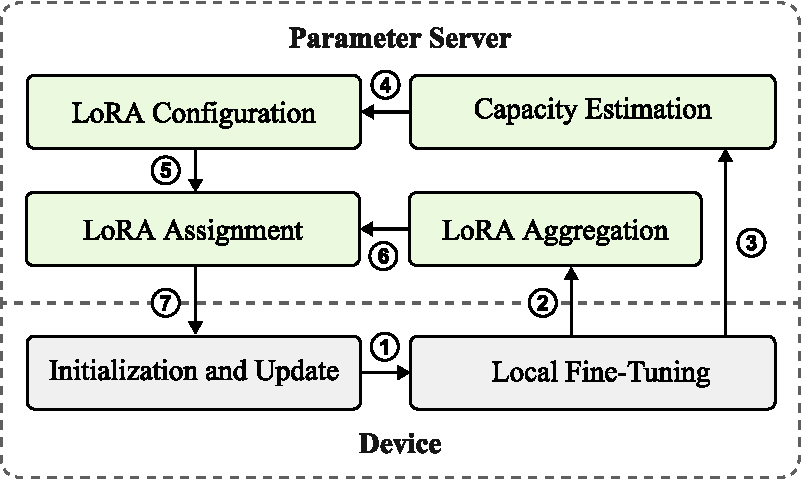
\includegraphics[width=1\columnwidth]{figs/system_overview.pdf}
    \vspace{-0.5cm}
    \caption{The proposed LEGEND framework. 
    }
    \label{framework}
\vspace{-0.4cm}
\end{figure}